%% % % % % % % % % % % % % % % % % % % % % % % % % % % % % % % % % % % % % % % % % % % % %%
%                OBSERVATORIO NACIONAL - MCT                              %
%                DEPARTAMENTO DE POS GRADUACAO                            %
%                PACOTE LaTeX PARA DISSERTACOES E TESES                                   % 
%                SET 2013                                                          		%
%                Este texto foi propositalmente digitado sem acentos!                     % 
% % % % % % % % % % % % % % % % % % % % % % % % % % % % % % % % % % % % % % % % % % % % % %

\documentclass[12pt,letterpaper]{report} %define o estilo do documento, tamanho da fonte, ...
%============================================================================================== %
%   %    %   MEUS DADOS
%============================================================================================== %
\newcommand{\meunome}{Autor}
\newcommand{\meutitulo}{Titulo}
\newcommand{\meusubtitulo}{Sub titulo}
\newcommand{\meuano}{ano}
\newcommand{\meuorientador}{ {Orientador } }
%\newcommand{\meucoorientador}{ {}}
\newcommand{\titulacao}{Mestre/Doutor/qualifica��o} % ou mestre!
\newcommand{\doctipe}{Disserta��o de Mestrado}%ou Dissertacao de Mestrado, tese de doutorado...
%============================================================================================== %
%   %    % %   %    % %   %   INICIO DOS PREAMBULOS     % %   %    % %   %    %    %    %  %    %
%============================================================================================== %


%============================================================================================== %
%   %    %   CODIFICACAO DO EDITOR LaTeX
%============================================================================================== %
% % % % % %  Habilite o correspondente ao seu tipo de Sistema/Editor.
% % % % % %  Em ambos voce pode digitar os acentos normalmente!

% ISO-8859-1 (WINDOWS usa este tipo de codificacao)
%           \usepackage[T1]{fontenc}
%           \usepackage{palatino}
            \usepackage[latin1]{inputenc}

% UTF-8    (LINUX usa geralmente este tipo de codificacao por default.)
	    \usepackage[T1]{fontenc} %usa caracteres especiais
%           \usepackage{type1cm}
%           \usepackage{ucs}
	    \usepackage{palatino}
%            \usepackage[utf8x]{inputenc} %usa caracteres acentuados diretamente  AQUIIIIIIIIII___LINUXXXXXXX
%============================================================================================== % 
% % % % % %  OBSERVACAO 1:
% % % % % %  Para mudar a codifica��o de um arquivo (no linux) use:
% % % % % %     iconv -f UTF-8 -t ISO-8859-1 arquivo_em_utf8.txt > novo_arquivo_em_latin1.txt
%============================================================================================== % 

             \usepackage[brazil]{babel} %define a linguagem - portugues brasil
%============================================================================================== % 
%   %    %   FORMATACAO BASICA DO EDITOR LATEX
%============================================================================================== %
             \usepackage{latexsym,amsmath,amssymb,amsfonts,textcomp,marvosym,wasysym}
             \usepackage{appendix}        	% pacote apendice
             \usepackage{epigraph}

%============================================================================================== %
%   %    %   USANDO LINKS SIMBOLICOS
%============================================================================================== %
% % % % % %  Escolha colorlinks=false ou colorlinks=true
             \usepackage{hyperref}
             \hypersetup{colorlinks=true, linkcolor=blue, citecolor=blue, filecolor=blue,
            pagecolor=blue, urlcolor=green,
            pdfauthor={AUTOR DO TRABALHO},
            pdftitle={TITULO DO TRABALHO},
            pdfsubject={TESE ou DISSERTACAO + ANO},
            pdfkeywords={PALAVRAS CHAVES},
            pdfproducer={LaTeX},
            pdfcreator={pdfLaTeX}} 
            \usepackage{lastpage}
%============================================================================================== %
%   %    %   ELEMENTOS GRAFICOS
%============================================================================================== %
            \usepackage[all,knot,arc,import,poly]{xy}
            \usepackage{picinpar}
            \usepackage[]{graphicx}	% Figuras (pacote extendid0)
            \usepackage{float}	
            \usepackage{color}				% Cores
            \usepackage[table]{xcolor}
            \usepackage{subfig}				% Criar figura dividida em subfiguras
            \graphicspath{{./figuras/}}		% Caminho para o diretorio das figuras
            \usepackage{caption}	        % Customizar as legendas das figuras e das tabelas
            \captionsetup[subfigure]{style=default, margin=0pt, parskip=0pt, 
				    hangindent=0pt, indention=0pt, singlelinecheck=true, 
				    labelformat=parens, labelsep=space}
            \usepackage{multicol}			% Criar ambientes em colunas
            \usepackage{verbatim}
%============================================================================================== %
%   %    %   TABELAS
%============================================================================================== %
            \usepackage{array}				% Elementos extras de formatacao
            \usepackage{booktabs}			% Tabelas com excelente qualidade 
            \usepackage{longtable}			% Para criar tabelas longas
            \usepackage{lscape}				% layout da pagina em landscape
%============================================================================================== %
%   %    %   NOTAS DE RODAPE 
%============================================================================================== %
            \usepackage{footnote}			% notas de rodape em geral
            \makesavenoteenv{tabular}		% Notas criadas nas tabelas ficam no fim das tabelas!

%============================================================================================== %
%   %    %  LAYOUT DA TESE: PAGINA
%============================================================================================== %
           \usepackage[Glenn]{fncychap}	   % 
           \usepackage{fancyhdr}           % configuracao para cabecalhos e rodapes

           \usepackage[dvips]{geometry}
           \usepackage{setspace}

           \geometry{left=30mm} 
           \geometry{right=20mm} 
           \geometry{top=30mm}
           \geometry{bottom=20mm} 
           \geometry{headheight=15pt}
           \geometry{headsep=10mm}                  % espaco entre paragrafo e cabecalho
           \geometry{footskip=10mm}                 % espaco entre par�grafo e rodape

           \linespread{1.3}
           \setlength{\parindent}{15mm}             % indentacao do paragrafo
           \setlength{\parskip}{6pt}                % espaco entre paragrafos
           \setlength{\abovecaptionskip}{5pt}       % espaco entre legenda e tabela ou grafico
           \setlength{\belowcaptionskip}{5pt}       % espaco entre legenda e tabela ou grafico
           % % % %           SECOES E SUBSECOES                % % % % % % %
           \setcounter{secnumdepth}{5}
           \setcounter{tocdepth}{3}
           
           % % % % NAO ENUMERAR A FOLHA QUE MARCA UMA NOVA PARTE% % % % % % %
           \makeatletter
           \let\sv@endpart\@endpart
           \def\@endpart{\thispagestyle{empty}\sv@endpart}
           \makeatother
           % % % % % % % % % % % % % % % % % % % % % % % % % % % % % % % % % %

%============================================================================================== %
%   %    %  LISTA DE ABREVIACOES
%============================================================================================== %
           %\usepackage[intoc,portuguese]{nomencl}	% Pacote que cria lista de abreviacoes
	   \usepackage[portuguese]{nomencl}	% Pacote que cria lista de abreviacoes
           \makenomenclature	                        % Comando para criar a lista
%============================================================================================== % 
% % % % % % OBSERVACAO 2: 
% % % % % %
% % % % % % Para poder criar a lista de simbolos e necessario fazer:
% % % % % % No linux: Abra o terminal, no diretorio onde se encontra seu arquivo .tex, digite:
% % % % % %         makeindex ON_form.nlo -s nomencl.ist -o ON_form.nls
% % % % % % Mas, Se vc tiver compilado diretamente no Terminal, com 
% % % % % %         pdflatex ON_form.tex
% % % % % % este comando acima torna-se desnecessario, pois o indice ja tera sido criado!
% % % % % % No Windows: Vc podera colocar este comando no RUN de seu editor TeX.
%============================================================================================== % 


%============================================================================================== %
%   %    %  CABECALHO E RODAPE
%============================================================================================== %
            \usepackage{fancyhdr}
            \fancyhead[LO,LE]{\textit\footnotesize\nouppercase\leftmark}
            \fancyhead[RO,RE]{\textit\footnotesize\nouppercase\thepage}
            \fancyfoot[CO,CE]{}
%============================================================================================== %
%   %    %  HIFENIZACAO CORRETA
%============================================================================================== %
          \hyphenation{e-xem-plos} %Coloce entre {} todas as palavras que nao forem corretamente

%============================================================================================== %
%   %    %  CRIANDO COMANDO PERSONALIZADOS 
%============================================================================================== %

            %\newcommand{\cao}{\c{c}\~ao }
            %\newcommand{\coes}{\c{c}\~oes }
            %\newcommand{\ii}{\'{\i}}

%============================================================================================== %
%   %    % %   %    % %   %   FIM DOS PREAMBULOS     % %   %    % %   %    %    %    % %   %    %
%============================================================================================== %


\begin{document}

%============================================================================================== %
%   %    %  LAYOUT DA TESE: MUDANDO O NOME DOS ELEMENTOS
%============================================================================================== %
           \renewcommand{\contentsname}{sum�rio}
           \renewcommand{\partname}{Parte}
           \renewcommand{\chaptername}{Cap�tulo}
           \renewcommand{\appendixname}{Apendice}
           \renewcommand{\bibname}{Refer�ncias}
           \renewcommand{\figurename}{Figura}
           \renewcommand{\listfigurename}{lista de figuras}
           \renewcommand{\tablename}{Tabela}
           \renewcommand{\listtablename}{lista de tabelas}
           \renewcommand{\nomname}{lista de siglas}   % Nomeia a Lista como Lista de Simbolos
           \renewcommand{\thefigure}{\thechapter.\arabic{figure}}
           \renewcommand{\thetable}{\thechapter.\arabic{table}}


%============================================================================================== %
%   %    %  ELEMENTOS PRE-TEXTUAIS
%============================================================================================== %

            \pagenumbering{roman}

            
%*****************************************************
% Disseta��o - capa.tex
%
%*****************************************************


\begin{titlepage}
\begin{center}

\begin{figure}[!h]
  % Requires \usepackage{graphicx}
\centering

\includegraphics[scale=0.7]{figuras/logoon.png}\\
\end{figure}

{\sc \large Observat�rio Nacional \\
Minist�rio da Ci�ncia e Tecnologia\\
Programa de Pos Gradua��o em Astronomia\\}
\vspace{4cm}



{\LARGE \sc \meutitulo}\\
\vspace{0.2cm}
{\sc \Large \meusubtitulo}
\vspace{1cm}


{\sc \Large \meunome}
\end{center}
\vspace{5cm}

\begin{center}
{\sc \Large Rio de Janeiro - RJ\\
\sc \Large \meuano}
\end{center}

\end{titlepage}


			%%% elemento obrigatorio
            %*****************************************************
% Disserta��o - contra-capa.tex
%
%*****************************************************

\begin{titlepage}

\begin{center}
{\sc \Large \meunome}
\vspace{5cm}



{\LARGE \sc \meutitulo}\\
\vspace{0.2cm}
{\sc \Large \meusubtitulo}
\end{center}
\vspace{1cm}


\begin{flushright}
\begin{minipage}[t]{11cm}
\textit{\textbf{\doctipe} apresentada ao Programa de
P\'os-Gradua\c{c}\~ao em Astronomia do Observatorio Nacional como 
requisito parcial para a obten\c{c}\~ao do grau de
\textbf{mestre/doutor} em Astronomia.}
\end{minipage}
\end{flushright}
\begin{flushright}
\begin{minipage}[t]{11cm}
\textbf{Orientador}: \meuorientador \\ 	
%\textbf{Co-orientador}: \meucoorientador
\end{minipage}
\end{flushright}

\vspace{4.5cm}

\begin{center}
{\sc \Large Rio de Janeiro - RJ\\
 \sc \Large \meuano}
\end{center}

\end{titlepage}		%%% elemento obrigatorio
%			*****************************************************
% Disserta��o - dedicatoria.tex
%*****************************************************
%\begin{tabular}{l}
%\hline \hline {\bf Para Pessoas Especiais:} \\ \hline \hline
%\end{tabular}

%\begin{flushright}
%\begin{minipage}[b][20cm]{10cm}
%\begin{flushright}
%fa�a a dedicat�ria auqi
%\end{flushright}
%\end{minipage}
%\end{flushright}
%\pagenumbering{roman}
		%%% elemento opcional
            %*****************************************************
% Disseta��o - agradecimento.tex
%*****************************************************
%\addcontentsline{toc}{chapter}{Agradecimento}
\begin{center}
{\LARGE\sc Agradecimentos}
\end{center}


Bla bla bla...		%%% elemento opcional
%            %%%%%%%%%%%%%%%%%%%%%%%%%%%%%%%%%%%%%
%% Epigrafe
%%%%%%%%%%%%%%%%%%%%%%%%%%%%%%%%%%%%%

			%%% elemento opcional
            %*****************************************************
% Disseta��o - resumo.tex
%*****************************************************

%\addcontentsline{toc}{chapter}{Resumo}

\begin{center}
{\Large\bf Titulo da tese/dissertacao} \\
\end{center}


\begin{center}
{\Large\bf Resumo} \\
\end{center}

O resumo e uma das partes mais importantes de uma tese ou artigo. Esforce-se para escrever bem de forma clara e objetiva.			%%% elemento obrigatorio
            %*****************************************************
% Disseta��o - abstract.tex
%*****************************************************
%\addcontentsline{toc}{chapter}{Abstract}

\begin{center}
{\Large\bf Title (make the tag to main title)} \\
\end{center}



\begin{center}
{\Large\bf Abstract} \\
\end{center}


The same as before.			%%% elemento obrigatorio

	    \clearpage
            \listoffigures % iclui a lista de figuras				%%% elemento opcional
            \addcontentsline{toc}{chapter}{\listfigurename}

            \clearpage
            \markboth{\nomname}{\nomname} 
            \printnomenclature            % aqui inclui a lista de siglas ou simbolos ou abreviacoes.	%%% elemento obrigatorio
        

            \tableofcontents % inclui o sumario
            \addcontentsline{toc}{chapter}{\contentsname}
            \newpage

%============================================================================================== %
%   %    %  ELEMENTOS TEXTUAIS
%============================================================================================== %
            \pagestyle{fancy}
            \pagenumbering{arabic}
            \newpage\pagebreak

            %%%%%%%%%%%%%%%%%%%%%%%%%%%%%%%%%%%%%%%%%%%%%%%%%%%%%%%%%%%%%%%%%
% Capitulo 0 - introducao
%%%%%%%%%%%%%%%%%%%%%%%%%%%%%%%%%%%%%%%%%%%%%%%%%%%%%%%%%%%%%%%%%


\chapter{Introdu��o}
%\addcontentsline{toc}{chapter}{Introdu��o}

\vspace{-1cm} 
~
\begin{flushright}
\begin{minipage}[t]{6cm}
\footnotesize\textit{Bla bla bla}\\
\rule[0.01mm]{6cm}{0.01mm}\\
\end{minipage}
\end{flushright}
\vspace{0.5cm}


\nomenclature{ON}{Observatorio Nacional - MCT}


\begin{figure}[!htb]
     \centering
     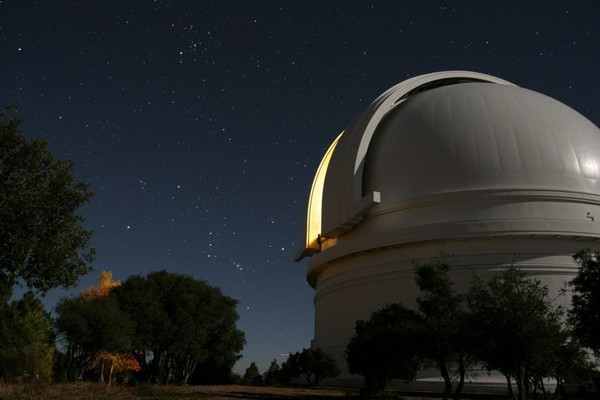
\includegraphics[scale=0.75]{figuras/palom1.jpg}
     \caption{Figura teste. O Caption que escreve aqui fica na figura}
     \label{O label que escreve aqui fica na lista de figuras.}
\end{figure}


            %%%%%%%%%%%%%%%%%%%%%%%%%%%%%%%%%%%%%%%%%%%%%%%%%%%%%%%%%%%%%%%%%
% Capitulo 2 - dados utlizados
%%%%%%%%%%%%%%%%%%%%%%%%%%%%%%%%%%%%%%%%%%%%%%%%%%%%%%%%%%%%%%%%%

\chapter{Dados utilizados}

\vspace{-1cm} 
~
\begin{flushright}
\begin{minipage}[t]{6cm}
{\footnotesize\textit{bla bla}}\\
\rule[0.01mm]{6cm}{0.01mm}\\
{\footnotesize Cebolinha}
\end{minipage}
\end{flushright}
\vspace{0.5cm}


			%%%%%%%%%%%%%%%%%%%%%%%%%%%%%%%%%%%%%%%%%%%%%%%%%%%%%%%%%%%%%%%%%
% Capitulo - Resultados
%%%%%%%%%%%%%%%%%%%%%%%%%%%%%%%%%%%%%%%%%%%%%%%%%%%%%%%%%%%%%%%%%

\chapter{metodos}

\vspace{-1cm} 
~
\begin{flushright}
\begin{minipage}[t]{6cm}
{\footnotesize\textit{Passam os s�culos e os homens mas repetem-se os fatos e suas causas.
"}}\\
\rule[0.01mm]{6cm}{0.01mm}\\
{\footnotesize  Gaspar Barlaeus}
\end{minipage}
\end{flushright}
\vspace{0.5cm}


Exemplo de tabela.

\begin{table}
\centering
\caption{Resumos dos resultado obtidos para o periodograma da varia��o temporal da profundidade da linha e uma lista dos per�odos obtidos em ordem de signific�ncia do sinal. $P_{Rot}$ � o per�odo de rota��o em dias e $^{*}$ representa as linhas que sofreram corre��o tel�rica.}
\label{compa}
\begin{tabular}{l|ccc}
\hline \hline \\[-2mm]	
elementos & $\lambda$ (\AA{}) & $P_{Rot}$ dias      &  $\sigma$  \\
\hline \\[-2mm]	



																
$Ti II$ & $5381.0$  & $27.87$  & $96.64$\\


\hline
\hline


\end{tabular}
\end{table}


			%%%%%%%%%%%%%%%%%%%%%%%%%%%%%%%%%%%%%%%%%%%%%%%%%%%%%%%%%%%%%%%%%
% Capitulo - Resultados
%%%%%%%%%%%%%%%%%%%%%%%%%%%%%%%%%%%%%%%%%%%%%%%%%%%%%%%%%%%%%%%%%

\chapter{Resultados}

\vspace{-1cm} 
~
\begin{flushright}
\begin{minipage}[t]{6cm}
{\footnotesize\textit{""}}\\
\rule[0.01mm]{6cm}{0.01mm}\\
{\footnotesize  Ramiro de la Reza}
\end{minipage}
\end{flushright}
\vspace{0.5cm}

Exemplo de tabela
...
			%%%%%%%%%%%%%%%%%%%%%%%%%%%%%%%%%%%%%%%%%%%%%%%%%%%%%%%%%%%%%%%%%
% Disserta��o - Conclus�o
%%%%%%%%%%%%%%%%%%%%%%%%%%%%%%%%%%%%%%%%%%%%%%%%%%%%%%%%%%%%%%%%%


\chapter{Conclus�es}
%\addcontentsline{toc}{chapter}{Introdu��o}

\vspace{-1cm} 
~
\begin{flushright}
\begin{minipage}[t]{6cm}
{\footnotesize\textit{""}}\\
\rule[0.01mm]{6cm}{0.01mm}\\
{\footnotesize }
\end{minipage}
\end{flushright}
\vspace{0.5cm}


\nomenclature{ON}{teste}

Conclusoes
			%%%%%%%%%%%%%%%%%%%%%%%%%%%%%%%%%%%%%%%%%%%%%%%%%%%%%%%%%%%%%%%%%
% Disserta��o - Perspectivas
%%%%%%%%%%%%%%%%%%%%%%%%%%%%%%%%%%%%%%%%%%%%%%%%%%%%%%%%%%%%%%%%%


\chapter{Perspectivas}
%\addcontentsline{toc}{chapter}{Introdu��o}

\vspace{-1cm} 
~
\begin{flushright}
\begin{minipage}[t]{6cm}
{\footnotesize\textit{" Oe yes"}}\\
\rule[0.01mm]{6cm}{0.01mm}\\
{\footnotesize Fulano de Tal}
\end{minipage}
\end{flushright}
\vspace{0.5cm}




perspectivas




%============================================================================================== %
%   %    %  ELEMENTOS POS-TEXTUAIS
%============================================================================================== %


           \appendix
           \renewcommand{\setthesection}{\Alph{section}}
           %%%%%%%%%%%%%%%%%%%%%%%%%%%%%%%%%%%%%%%%%%%%%%%%%%%%%%%%%%%%%%%%%
% Dissertacao - Apendice
%%%%%%%%%%%%%%%%%%%%%%%%%%%%%%%%%%%%%%%%%%%%%%%%%%%%%%%%%%%%%%%%%


\addcontentsline{toc}{chapter}{Ap�ndices}

\chapter{Apendice}  %\label{efstark}


	   			%\include{apendb}
            
            \clearpage
            \listoftables  %inclui a lista de tabelas				%%% elemento opcional
            \addcontentsline{toc}{chapter}{\listtablename}
\begin{flushright}
\begin{flushright}

\end{flushright}
\end{flushright}

           %%%%%%%%%%%%%%%%%%%%%%%%%%%%%%%%%%%%%%%%%%%%%%%%%%%%%%%%%%%%%
% Bibliografia
%%%%%%%%%%%%%%%%%%%%%%%%%%%%%%%%%%%%%%%%%%%%%%%%%%%%%%%%%%%%%


\addcontentsline{toc}{chapter}{Referencias Bibliograficas}
\begin{thebibliography}
%%%%%%%%%%%%%%%%%%%%%%%%%%%%%%%%%%%%%
%%%%%%%%%%%%%%%%%%%%%%%%%%%%%%%%%%%%%%
%Bibliografia segundo normas da ABNT
%%%%%%%%%%%%%%%%%%%%%%%%%%%%%%%%%%%%%%
%%%%%%%%%%%%%%%%%%%%%%%%%%%%%%%%%%%%%%
%Exemplo 1
%livro com um autor
%Autor. Título; Subtítulo. Edição Local: Editora, Ano

\bibitem{1}
Poster 71.\\


\end{thebibliography}

\end{document}